\documentclass[fleqn]{article}
\usepackage{amsmath}
\usepackage[margin=0.25in]{geometry}
\usepackage{siunitx}
\usepackage{graphicx}
\usepackage{caption}
\usepackage{subcaption}
\usepackage[thinc]{esdiff}
\usepackage{pgfplots}
\usepackage{esdiff}
\usepackage{indentfirst}
\usepackage{multicol}
\pgfplotsset{width=10cm,compat=1.9}
\usepgfplotslibrary{external}
\usepgfplotslibrary{fillbetween}
\tikzexternalize
\graphicspath{{./}}
\renewcommand{\arraystretch}{1.5}

\begin{document}

\title{6.S092 Final Report: Amateur Radio Satellite Phased Array Receive System}
\author{Oliver Trevor}
\date{February 3, 2021}
\maketitle

\section{Schematic}
\centerline{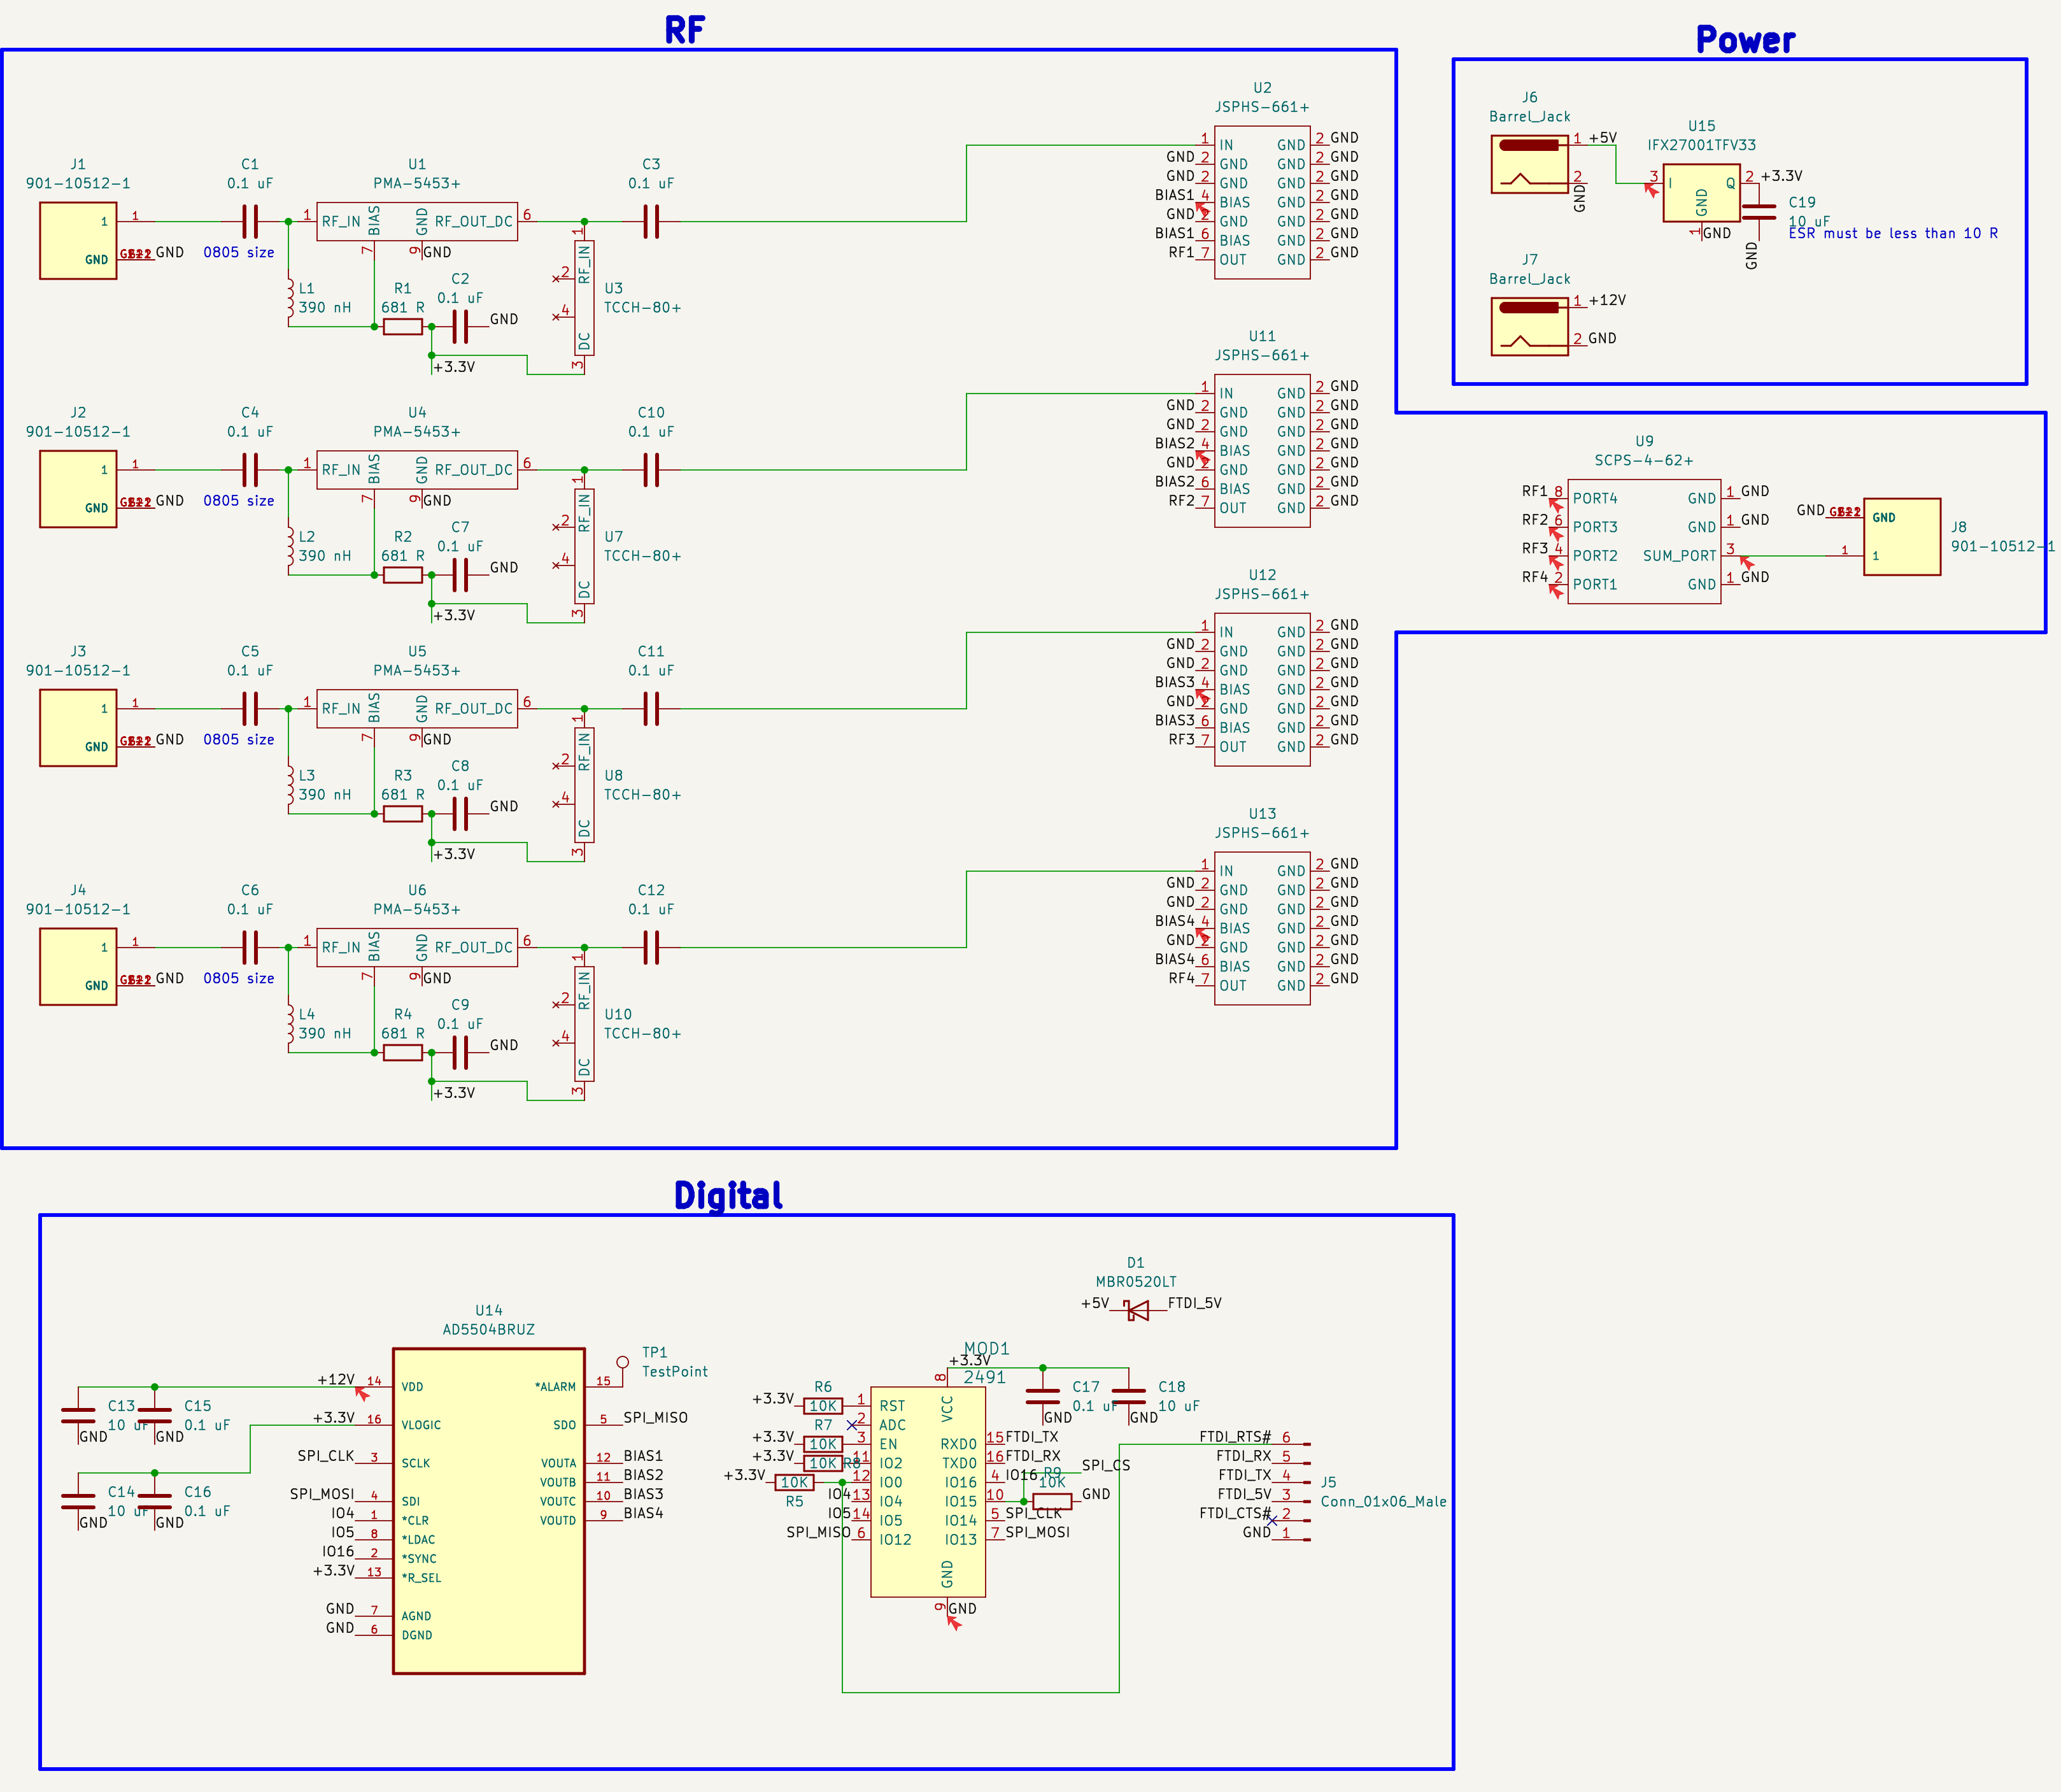
\includegraphics[width=8.25in]{schematic.png}}

\section{Layout and 3-D Rendering}
\centerline{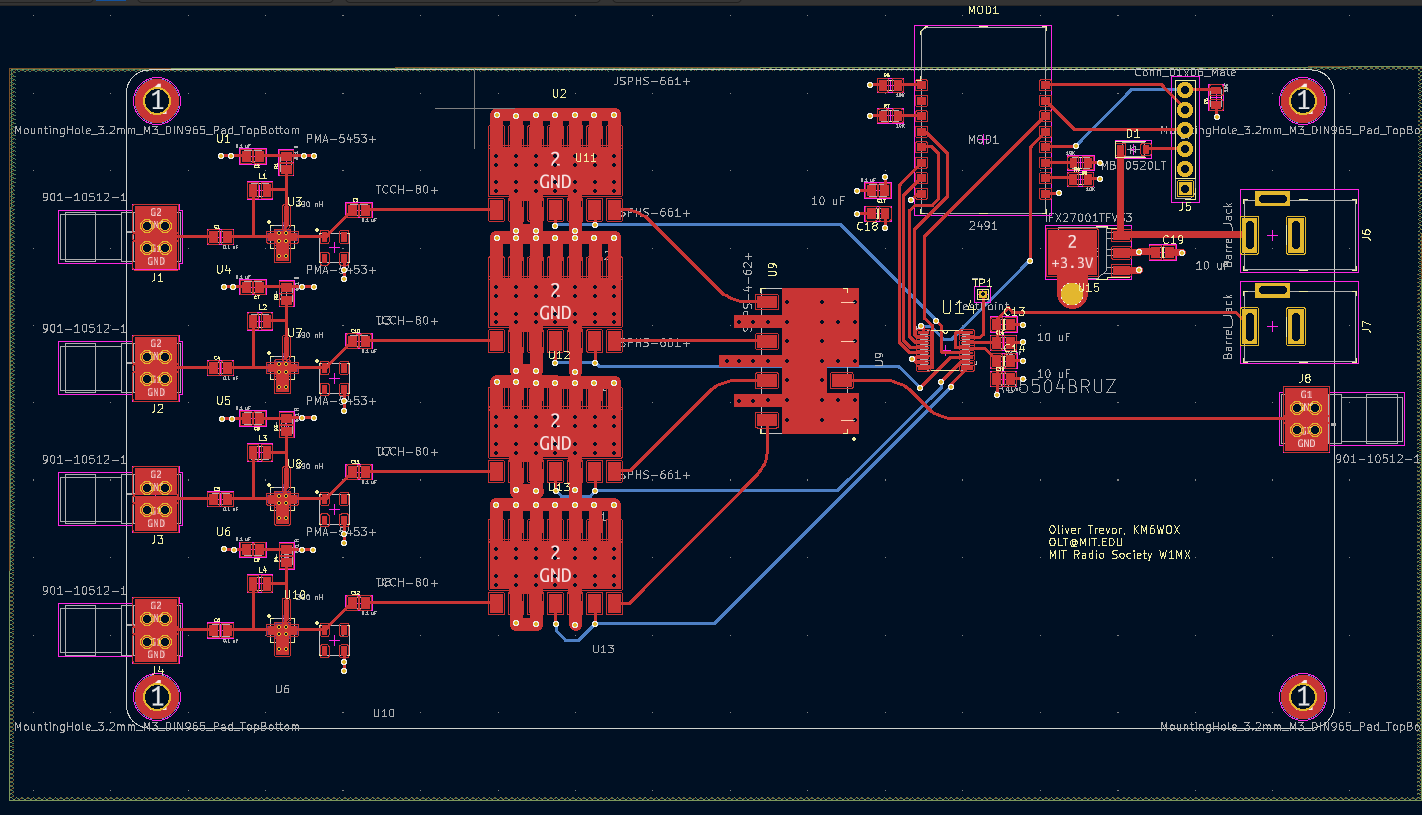
\includegraphics[width=8.25in]{layout.png}}
\centerline{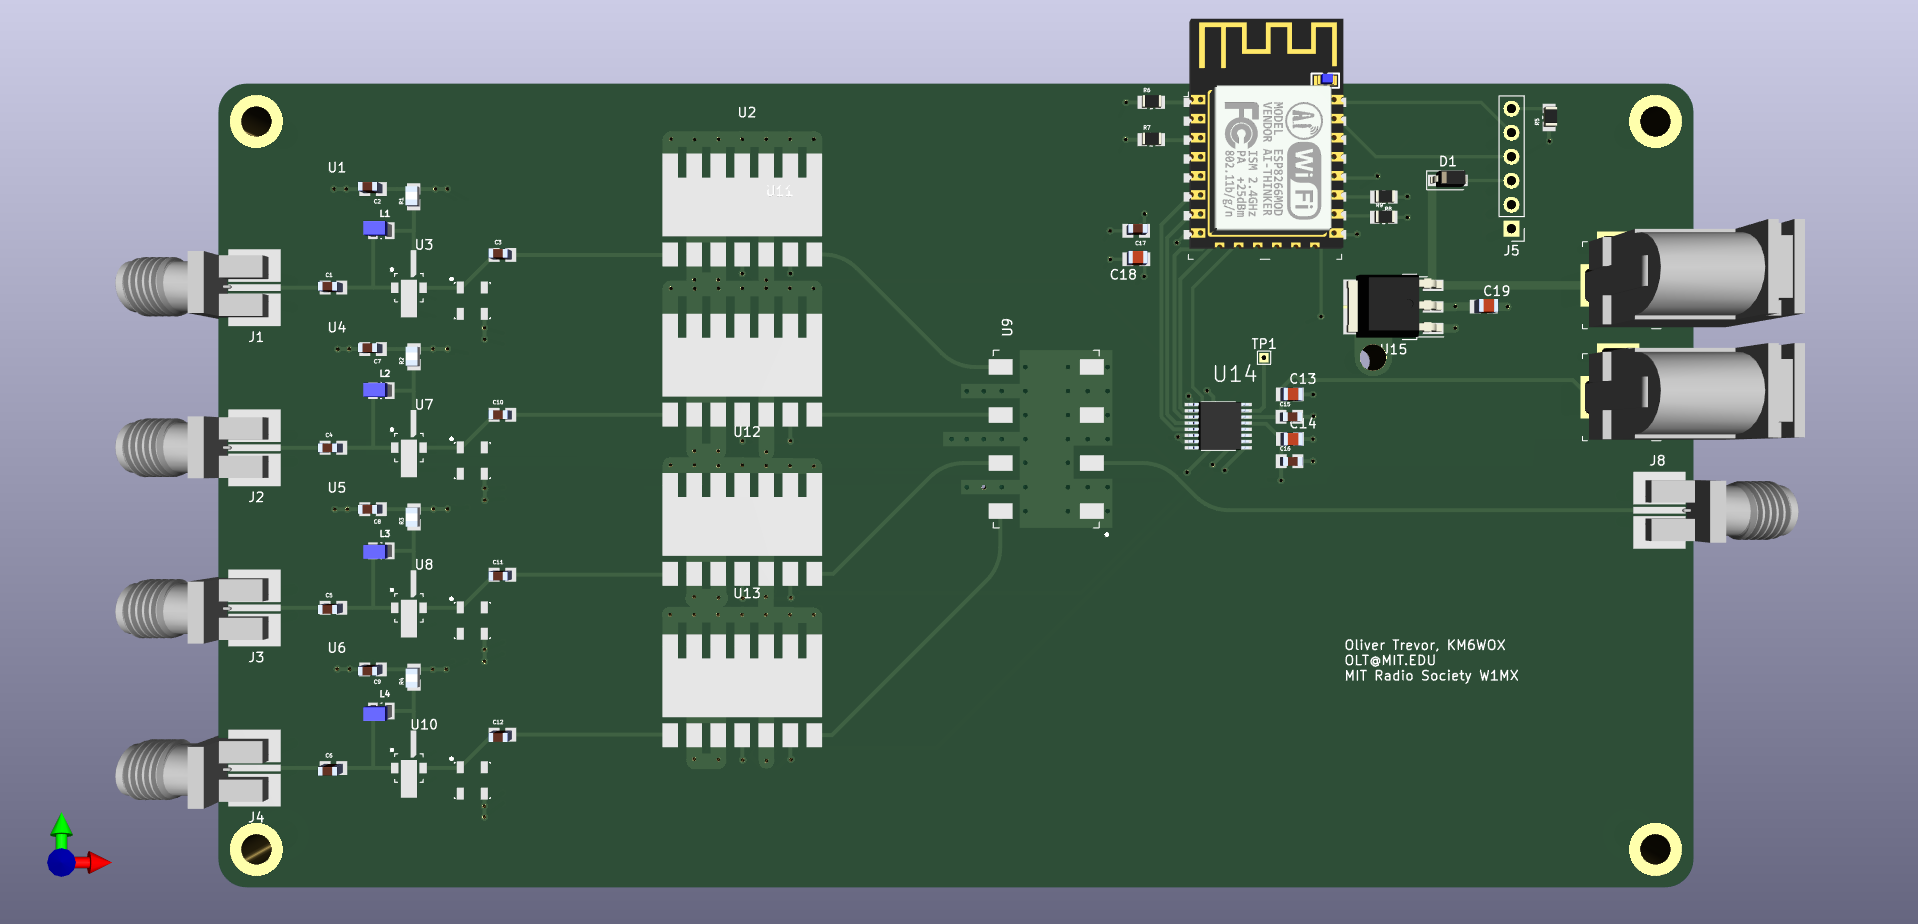
\includegraphics[width=8.25in]{3drender.png}}

\section{Background}

There are many small satellites in Earth orbit with amateur radio payloads, usually either cross-band repeaters for rebroadcasting amateur transmissions or data beacons. Since small CubeSats have limited power and volume (and are very far away), reliably receiving their signals requires a directional antenna and a low-noise amplifier. Most current amateur radio satellite systems use mechanically-steered antennas, where a motor physically points the antenna in the direction of the satellite being tracked. This limits slew speed and is prone to mechanical failure, especially with wind-loading and other environmental considerations.

The modern way of \emph{electronically} steering an antenna array, an ``electronically-steered phased array," works by altering the phase relationships between signals such that their constructive and destructive interference pattern produces a ``beam" in the desired direction. The well-known Starlink satellite Internet system partially uses an electronically-steered phased array (it also uses mechanical steering).

\section{Purpose and Requirements}

The goal of this project was to design a relatively inexpensive board for receiving the UHF (437 MHz) downlink signals from amateur radio satellites with a phased array of four antennas. The board should be usable with a regular, single-channel-receive ham radio (so the phase manipulation has to occur in the analog domain).

Additionally, the board should not require external amplification or impedance matching and should produce a signal that is safe to feed directly into a radio. The phase steering should be computer-controllable for use with satellite-tracking software.

\section{Design Choices}

\subsection{RF Chain}

Given the enormous path loss between a weak non-directional transmitter in Earth orbit and the ground (and the noise/losses introduced by the analog processing), amplification is necessary as the very first stage of the RF chain. I chose a surface-mount low-noise amplifier from Mini-Circuits that had the lowest noise factor and highest IP3 (intermodulation, a measure of linearity) for my frequencies of interest. The PMA-5453+ LNA has quite wide bandwidth, so, depending on local conditions, external filtering between the antennas and PCB may be necessary (although talking to a CubeSat researcher suggested that it wouldn't make much difference). I closely followed Mini-Circuits recommended design for the footprint and bias tee circuitry surrounding their LNA.

After being amplified by the LNA, the four signals from the antennas must be independently phase-shifted by independently-controllable amounts (this allows for steering the ``beam"). Electronically-controlled RF phase shifts in a small package are quite difficult to implement without creating impedance mismatches. Luckily, Mini-Circuits offers a voltage-controlled phase shifter module called the JSPHS-661+. It requires only a 0-12V analog control signal to manipulate the phase shift. This also has internal matching circuitry, so no external complexity other than matched-impedance traces is required. The voltage-controlled phase shifters are the only part of the RF chain that does not have enough bandwidth to also cover satellites with a VHF downlink (so the board can be used on VHF by switching to a different phase shifter).

The output of the phase shifters feeds into a Mini-Circuits power splitter/combiner module being used as a combiner called the SCPS-4-62+, which was chosen specifically for its low phase and amplitude unbalance, which is important because we are trying to superimpose the signals with the exact phase relationship created by the phase shifters.

The power combiner output is routed straight to an SMA port that can be connected to a radio.

\subsection{Analog Circuitry}

I was initially intending to use a 4-channel DAC with a quad op-amp to get the 0-12V range necessary, but I was instead able to find a specialized ``high-voltage DAC" chip that includes its own amplification, which simplified the layout significantly. The AD5504BRUZ DAC chip also has its own internal reference, so I did not need to add an external voltage reference. The non-linear relationship between control voltage and phase shift in the JSPHS-661+ means that software calibration will still be required, though.

3.3V power comes from an LDO that down-regulates it from the 5V DC power jack. Keeping switching converters off the PCB is good because they make a lot of RF noise.

\subsection{Microcontroller}

I chose an ESP8266 module mostly because a) they are available because people don't want to use them as much anymore and b) it gives me the option of wireless control and c) I have done the layout for one before and didn't want to risk having to manufacture multiple iterations of a \$300 RF board just because the digital part was wrong. The ESP8266 communicates with the DAC over SPI.

Plugging an FTDI cable onto a 6-pin header lets you program and communicate with the ESP8266. Not using an FTDI chip lets us dodge the chip shortage and avoid the added layout complexity.

\subsection{Layout Considerations}

Microstrip transmission lines require a solid ground plane very close to the top layer (otherwise the trace width required to make 50 Ohm transmission lines becomes very large), so a 4-layer board is necessary.

Grounding is very important for RF components, so the RF modules all have lots of ground pins and lots of ground vias to create a very low-impedance path to ground.

3.3V power is routed through another solid plane, and control signals are routed on the back of the board.

KiCad's PCB calculator let me determine what trace width to use to create 50 Ohm microstrip transmission lines with OSH Park's 4-layer FR4 stackup. Curved/smooth traces were used for the RF routing to avoid sharp corners acting as antennae.

\newpage

\subsection{Resources Used}

\begin{figure}[h]
    
\includegraphics[width=5in]{anime_deesh.jpg}
    \caption{Anime Deesh}
\end{figure}

Also thank you to Daniel DeSantis and Joey Murphy for all the help in the Radio Society chat with RF PCB design and satellite communications stuff, neither of whom I have anime versions of to include here.

Thanks to Adi and Fischer for teaching the class!

And thanks to Will Vu for advice about RF PCB design.

\end{document}
